\chapter{Marco teórico}\label{chapter:background}

En este capítulo se introducen conceptos de Aprendizaje Automático (AA). Temas
como la representación de datos, arquitecturas y evaluación de modelos son tratados en sus secciones.
Luego, se hace un recorrido por las diferentes investigaciones recientes realizadas en la EA, viendo
los enfoques desarrollados y la evolución de estos a partir del desarrollo e introducción de nuevos métodos en el
campo. Por último, se introduce la proyección de corpus, técnica necesaria para la creación de conjuntos 
de datos para el entrenamiento de modelos de AA.

\section{Aprendizaje Automático}

Existen varios problemas para los cuales es difícil escribir un programa de forma tradicional que pueda
resolverlo, por ejemplo, decir si en una imagen existe un gato o un perro, o transcribir una grabación. En el caso
de que se escribiera este programa probablemente sería frágil y poco escalable. El AA constituye el 
estudio de técnicas que pueden aprender de la experiencia [\cite{d2l}] y mediante su uso 
se puede automatizar el proceso de encontrar soluciones a dichos problemas, haciendo que sus resultados sean 
robustos y escalables. 

En AA existen tres tipos de aprendizaje:
\begin{itemize}
	\item Aprendizaje no supervisado: trabaja con datos no anotados y los algoritmos tratan de 
	extraer información de estos.
	\item Aprendizaje reforzado: trabaja en la creación de agentes que interactúen con 
	un ambiente obteniendo información de qué tan buenas son las acciones realizadas.
	\item Aprendizaje supervisado: trabaja con datos anotados y los algoritmos tratan de minimizar
	el error cometido en las predicciones.
\end{itemize}
A este último principalmente se refiere esta sección.

Los componentes básicos de un problema de aprendizaje supervisado se pueden resumir en los datos de los que 
aprender, el modelo para transformar los datos, una función de pérdida que cuantifica qué tan malo o bueno es el 
modelo y un algoritmo que ajuste los parámetros del modelo para minimizar la pérdida.

Matemáticamente, un modelo constituye una función $\hat{y} = f_{\theta}(x)$ cuyo argumento son las 
representaciones de las entradas originales $x$ y devuelve una salida $\hat{y}$. Esta función $f$ se encuentra
parametrizada por el vector $\theta$ el cual constituye los parámetros en los que el modelo se basa para realizar sus
cálculos. La función de pérdida se puede definir como $e(y, \hat{y})$, donde $y$ es el resultado esperado para $x$. 
El objetivo final del algoritmo de ajuste es encontrar $\theta$ tal que:

\begin{equation}
	\arg \min_{\theta} e(y, f_{\theta}(x)).
\end{equation}\label{eq:arg_min_theta}

Los parámetros $\theta$ eventualmente se van ajustando con algún algoritmo de optimización para que 
la función de error alcance un valor óptimo, aunque un óptimo global en la práctica es difícil de conseguir
debido a la complejidad del espacio de búsqueda.

Una manera de observar la complejidad de estos modelos sería la cantidad de capas de procesamiento que lo integran.
Los primeros modelos empezaron utilizando una sola capa\footnote{A estos modelos se les conoce 
como \emph{shallow} o poco profundos.} para realizar 
las tareas, más tarde estos modelos fueron ganando en complejidad al superponerle otras, dando paso al 
aprendizaje profundo (\emph{Deep Learning}). La superposición se refiere
a la composición de funciones $f_i$ y $f_{i+1}$ de tal forma que la imagen de $f_i$ sea compatible con el dominio de 
$f_{i+1}$, entonces se obtiene $f_{i+2}(x) = f_{i+1}(f_i(x))$, al aplicar este esquema se pueden agregar múltiples
capas y profundizar $f$ tanto como se desee.


\subsection{Representación de datos}

La representación de los datos constituye una parte importante al modelar un problema. Esta 
es la encargada de presentar datos abstractos, como imágenes, párrafos o sonidos, en formas tratables
por los algoritmos. Generalmente, se buscan configuraciones que recojan la mayor cantidad de información 
de la entrada relevante al problema.

En el PLN los datos suele estar representados con distintos niveles de granularidad.
De menor granularidad a mayor se pueden ir mencionando los documentos, párrafos, oraciones, palabras y
caracteres. Estos elementos es posible representarlos mediante vectores que codifiquen propiedades
objetivas del problema a tratar como características morfológicas o semánticas de estos. Por ejemplo, 
los textos tienen una popular manera de representarse mediante vectores de TF-IDF [\cite{manning2008introduction}],
una desventaja de esta representación es que no toma en cuenta el orden de las palabras, por lo que 
la representación de \emph{no me gusta,} y \emph{no, me gusta} serían iguales aunque semánticamente 
sean opuestas. Para agregarle la información de orden a la representación se introducen los llamados 
$n-$gramas, los cuales toman en cuenta una ventana de tamaño $n$ para conformar conjuntamente una representación.
Este enfoque conlleva a la limitante de que solo un contexto finito está disponible para hacer las inferencias,
para esto finalmente se crean representaciones individuales para cada palabra, las cuales codifican 
información y la secuencia completa es introducida al modelo para realizar la inferencia.
La manera más simple de representar una palabra es mediante la representación \emph{one-hot}, 
en esta, a cada palabra se le asigna un índice y el vector resultante posee la dimensión del 
vocabulario y es rellenado con ceros en todos sus elementos excepto en el índice de la palabra, donde se le asigna 1.
Esta representación asume que las palabras son independientes entre sí y 
computacionalmente ocupan un espacio considerable. Existen otras representaciones 
que brindan información al algoritmo sobre la morfología y la semántica de la palabra que representa.

Las características morfológicas son aquellas que describen cómo está formado el elemento a analizar.
Estas pueden ser extraídas con relativa facilidad, entre tales características se encuentran: tamaño, 
cantidad, posición de palabras o párrafos, presencia de sufijos, prefijos, acentos u otros marcadores
en el texto. Las características semánticas presentan una mayor dificultad a la hora de ser extraídas.
Para esto se utilizan diferentes modelos que codifican esta información en vectores continuos conocidos como 
\emph{embeddings}, entre los modelos existentes se encuentran
word2vec [\cite{mikolov2013efficient}], 
\emph{Global Vectors} (GloVe) [\cite{pennington2014glove}], 
\emph{Bidirectional Encoder Representations from Transformers} (BERT) [\cite{devlin2018bert}],
entre otros.

\subsection{Modelación de problemas}

Los problemas en la vida real se presentan en un principio como una descripción a un nivel de abstracción 
más alto que el requerido por los algoritmos existentes, se hablan de entidades abstractas como imágenes,
sonidos, textos o usuarios, además de la información que se desea extraer o las operaciones que se
desean aplicar sobre estas entidades. A lo largo del desarrollo del AA han aparecido diferentes tipos de problemas 
que aparecen frecuentemente en la práctica y sus respectivas maneras de solucionarlos. Uno de estos tipos de problemas
es el de secuencia a secuencia (\emph{seq2seq}), cuyo objetivo es la conversión de una secuencia en un dominio de entrada a otra 
secuencia en un dominio de salida. Con este tipo de problemas se modelan tareas como traducción automática, en 
donde el dominio de entrada es texto en un lenguaje de partida y el dominio de salida es texto en un lenguaje de llegada.
Otro problema que se resuelve con \emph{seq2seq} es la segmentación de texto, cuya entrada es una lista de \emph{tokens}
y la salida son etiquetas que indican cuándo empieza y termina un segmento de texto. Las etiquetas utilizadas para 
la segmentación, generalmente, son:

\begin{itemize}
	\item B (\emph{begin}): representa el inicio del segmento.
	\item I (\emph{inside}): representa la continuación del segmento previamente iniciado.
	\item O (\emph{outside}): representa la no pertenencia a un segmento.
\end{itemize}

Este esquema presenta una versión más elaborada en la que se agregan dos clases que representan el final 
de un segmento E (\emph{end}) y un segmento de un solo elemento S (\emph{single}). La tarea anterior es 
utilizada como base para otra un poco más compleja, en la que, además de segmentar el texto, se desea 
clasificar sus segmentos. Para este problema se añaden meta etiquetas correspondientes a los tipos a identificar $C$ 
% TODO Anotación {no dices quien es O} se dice arriba: representa la no pertenencia a un segmento.
obteniendo un conjunto final $R = \{ B, I, E, S \} \times C \cup \{ O \}$. En tareas como la extracción de entidades
nombradas este método es empleado, donde el conjunto $C$ contiene las posibles categorías de entidades a identificar.

\subsection{Arquitecturas}

En aprendizaje profundo existen una gran cantidad de arquitecturas que se pueden utilizar para formar el modelo 
final. Estas deben de ser seleccionadas en dependencia de los datos y el problema a tratar, ya que sus diseños 
emulan diferentes operaciones sobre datos que pueden ser más beneficiosas en situaciones específicas.

\subsubsection{Capas densas}

El perceptrón consiste es una transformación lineal del vector de datos $\textbf{x}$ con un sesgo $b$ y 
luego aplicar una transformación no lineal $g$, conocida como función de activación, 
para la obtención del resultado final:

\begin{equation}
	f(\textbf{x}) = g(\textbf{w}\textbf{x} + b).
\end{equation}

El perceptrón constituye la unidad básica de las capas densas, ya que estas consisten en la aplicación
de este modelo varias veces sobre la misma entrada $\textbf{x}$ produciendo vectores de la dimensión $k$ 
deseada como salida final. Los parámetros se codifican en la matriz $\textbf{W}$ y sus sesgo en el 
vector $\textbf{b}$:

\begin{equation}
	f(\textbf{x}) = g(\textbf{Wx} + \textbf{b}).
\end{equation}

Para las funciones de activación existen varias elecciones. Una de estas es la función sigmoidal. 
Esta devuelve un valor entre 0 y 1, es usada en tareas de regresión logística. 
Se puede interpretar como el nivel de activación de la neurona:

\begin{equation}
	sigm(x) = \frac{1}{1-e^{-x}}.
\end{equation}

\emph{Rectified Linear Unit} (ReLU) se define como la parte positiva del argumento. Una ventaja que trae esta 
función de activación es su rápido cálculo de su derivada y que previene en parte de los problemas 
de desaparición de gradiente de la sigmoidal:

\begin{equation}
	relu(x) = \max(0, x).
\end{equation}

La función de activación \emph{softmax} es diferente a las anteriores en el sentido que necesita
el vector salida de la capa anterior para ser computada. Esta función convierte las $q$ salidas
en una distribución de probabilidad, algo necesario en tareas de clasificación:

\begin{equation}
	softmax_k(\textbf{x}) = \frac{e^{x_k}}{\sum\limits_{i=1}^{q} e^{x_i}}.
\end{equation}

\subsubsection{Redes Neuronales Convolucionales}

Las redes neuronales convolucionales (CNN, en inglés) 
son un tipo de redes usadas
principalmente para tratar datos donde su estructura espacial es relevante, por ejemplo,
en datos bidimensionales como imágenes y en unidimensionales como sonido y texto.
Estas redes aplican de una función de kernel sobre los datos, $f * g$ donde $f$ son los
datos, $g$ es el kernel o filtro y $*$ es el operador de convolución [\cite{d2l}]. La función $g$ se puede 
aprender en el proceso o también puede ser una función de agrupación predefinida. 
Un ejemplo bidimensional de una función de kernel se muestra en la Figura \ref{fig:conv_kernel}.

\begin{figure}[h!]
	\begin{center}
		\begin{center}
			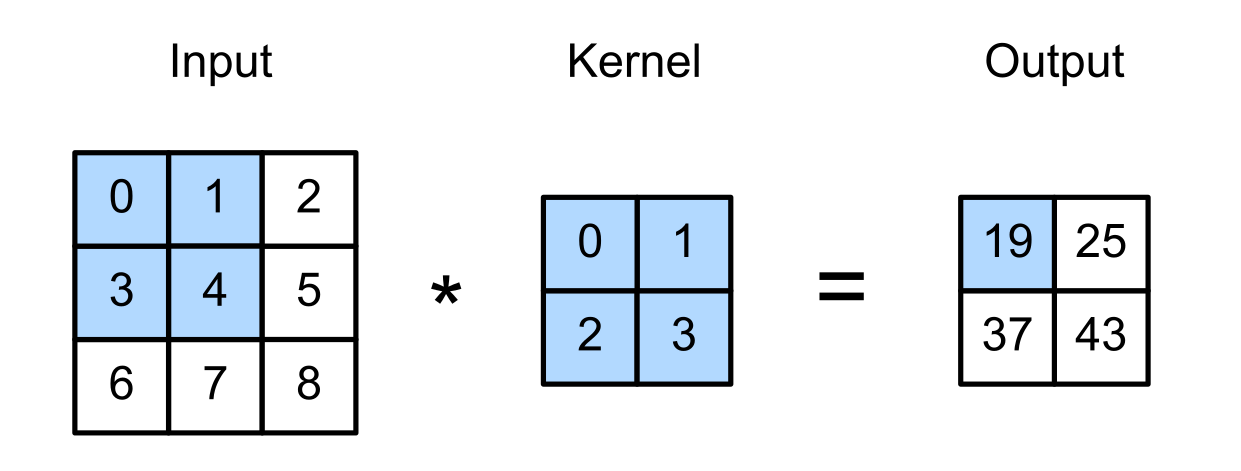
\includegraphics[scale=.4]{Graphics/kernel_convolution.png}
        \end{center}
		% TODO Cite problem, citar como texto
		% [\autocite{d2l}] 
		% [\parencite{d2l}] 
		% [\citet{d2l}] 
		% [\citep{d2l}] 
	    \caption{Convolución con kernel (Tomado de \textcite{d2l} pág. 241).}\label{fig:conv_kernel}
	\end{center}
\end{figure}

En este se observa cómo una nueva representación es computada al operar el kernel por la matriz de datos. Este
corrimiento se puede realizar de diferentes formas, por ejemplo, se puede mover de dos en dos en vez de uno en uno, este
parámetro se le conoce como tamaño de paso (\emph{stride}). Es posible además preservar las dimensiones
iniciales de los datos al aplicarle un aumento de los datos en los bordes de tal forma que el resultado sea de la misma
dimensión, este aumento se realiza, generalmente, rellenando convenientemente los espacios con ceros, 
a esto se le llama \emph{padding} (Figura \ref{fig:conv_kernel_padding}).

\begin{figure}[h!]
	\begin{center}
		\begin{center}
			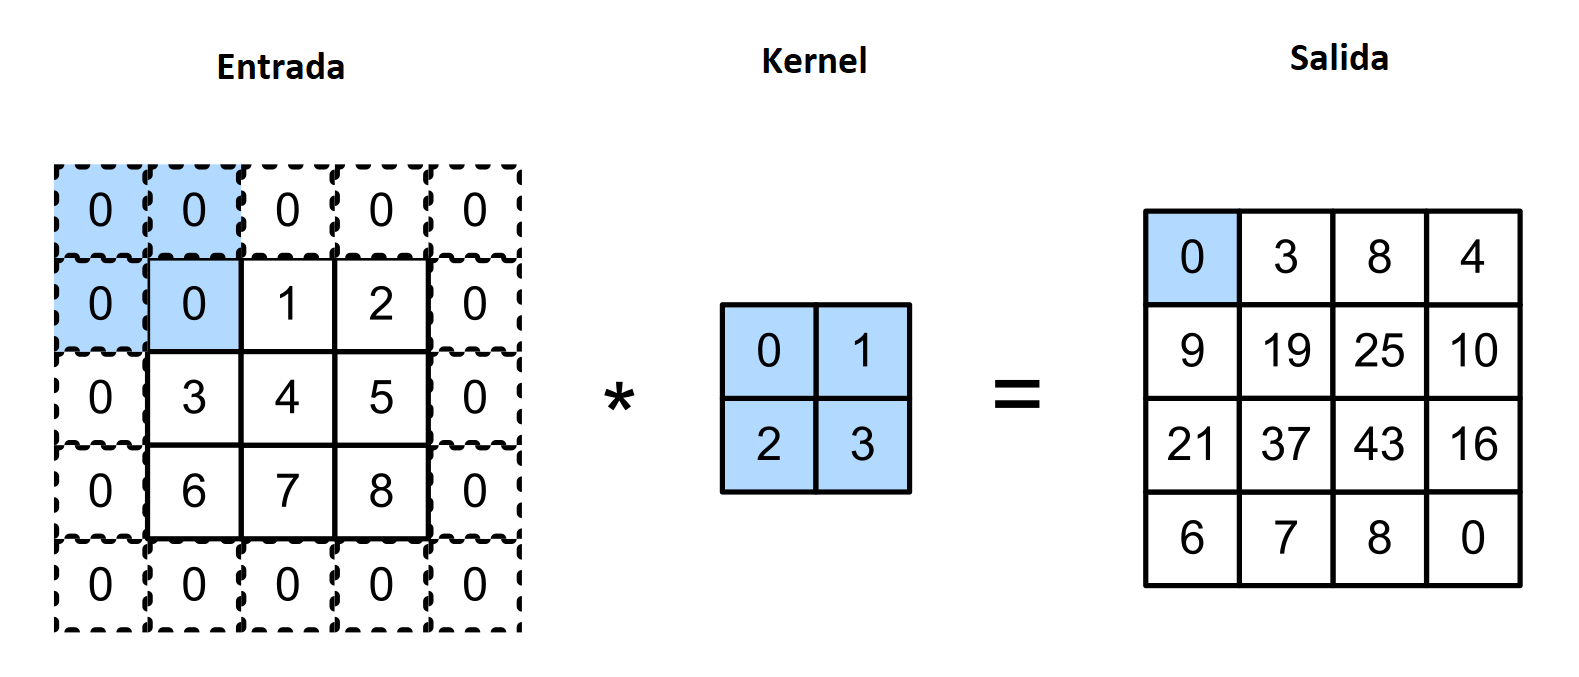
\includegraphics[scale=.4]{Graphics/kernel_convolution_padding.png}
        \end{center}
		% TODO Cite problem, citar como texto
		% [\autocite{d2l}] 
		% [\parencite{d2l}] 
		% [\citet{d2l}] 
		% [\citep{d2l}] 
		\caption{Convolución con kernel con \emph{padding} (Tomado de \textcite{d2l} pág. 241).}\label{fig:conv_kernel_padding}
	\end{center}
\end{figure}

Existen varias funciones de agrupación usadas. Entre estas se encuentran las de agrupación máxima y de 
agrupación media. Como sus nombres indican, la de agrupación máxima devuelve el valor máximo de los encontrados
en la ventana del kernel, la de media calcula el promedio de estos valores. Estas capas tienen la capacidad de obtener
información resumida sobre los datos.

\subsubsection{Redes Residuales}

Al crear modelos de aprendizaje profundo se tienen un conjunto de parámetros $\theta$. Las posibles combinaciones 
de estos forman un espacio de funciones $F$ al cual pertenecen todas las posibles instancias del modelo.
Agregar nuevas capas aumenta la complejidad de este, pero no hay garantía de que el viejo espacio 
de funciones $F$ sea subconjunto del nuevo espacio $F'$, lo que implica que el nuevo modelo no es necesariamente
estrictamente superior al antiguo. Este problema es la razón para la aparición de las Redes Residuales. 
Una red residual está formada por 
uno o varios bloques residuales, en los que a la salida de cada bloque residual le es sumada la entrada de 
este mediante una conexión residual.
El objetivo de realizar tal operación es que es posible hacer la contribución del bloque 0 obteniendo así
un modelo equivalente a uno sin el bloque, garantizando la condición de subconjunto $F \subset F'$, además,
dicho bloque no pierde poder expresivo, dado que en caso de que su aporte al resultado final sea considerable, 
se tendría que aprender solamente la función $f(x) - x$ donde $x$ es la entrada del bloque y $f$ es la función 
aprendida por el bloque sin la conexión residual, para mitigar el efecto de la conexión residual como se muestra
en la Figura \ref{fig:res_block}.

\begin{figure}[h!]
	\begin{center}
		\begin{center}
			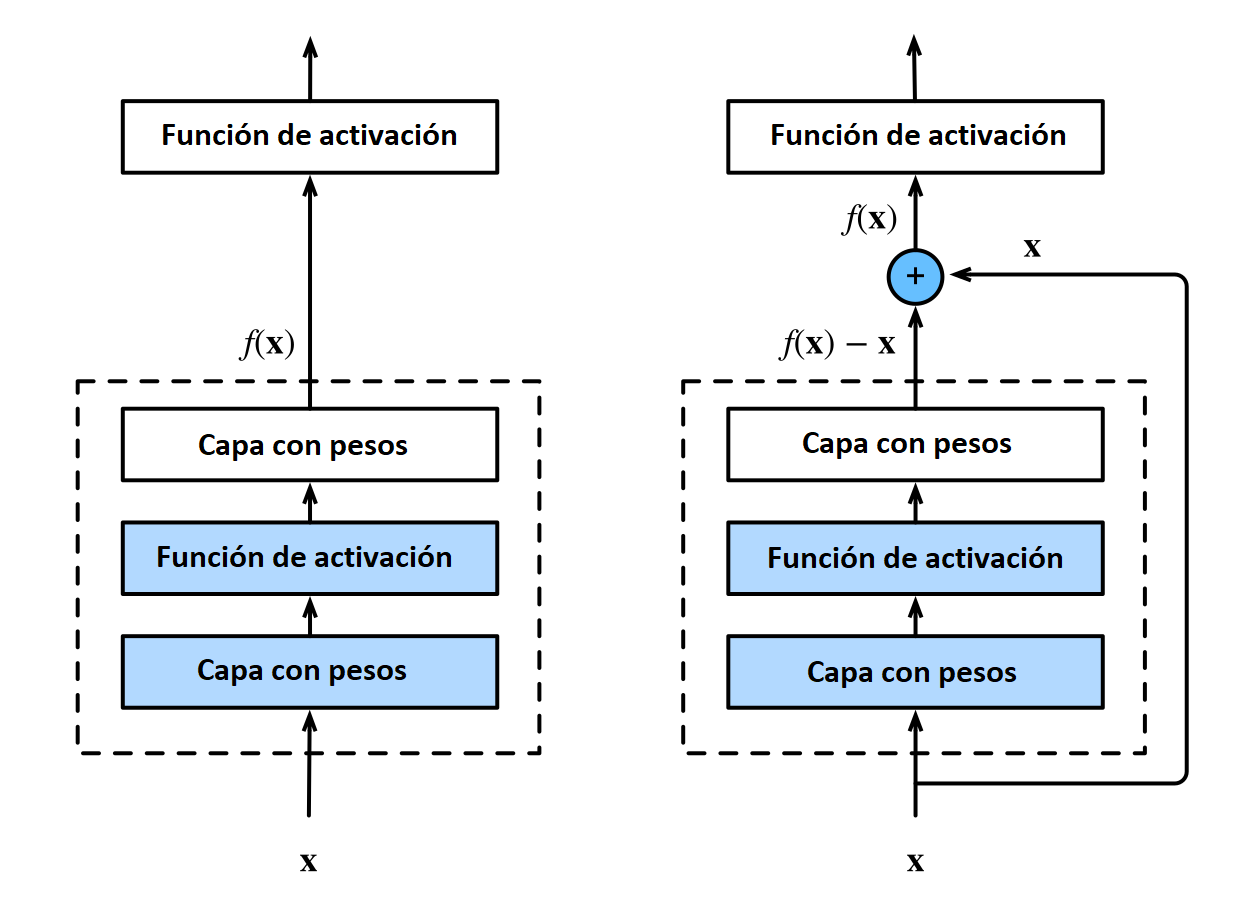
\includegraphics[scale=.4]{Graphics/resnet.png}
        \end{center}
		% TODO Cite problem, citar como texto
		% [\autocite{d2l}] 
		% [\parencite{d2l}] 
		% [\citet{d2l}] 
		% [\citep{d2l}] 
	    \caption{Bloque residual (Tomado de \textcite{d2l} pág. 289).}\label{fig:res_block}
	\end{center}
\end{figure}

\subsubsection{Redes Neuronales Recurrentes}

Las redes neuronales recurrentes (RNN, en inglés) son
un tipo especial de arquitectura especializada en el trabajo con datos secuenciales. Este tipo de arquitectura
presenta variables en las que se almacenan información pasada, que es usada para el computo de la salida. El 
problema se puede modelar probabilísticamente mediante la estimación de $P(x_t | x_{t-1}, \dots, x_{1})$,
donde existen dos variantes principales. En una variante se fija un tamaño de ventana $\alpha$ en el tiempo, 
dando como resultado $P(x_t | x_{t-1}, \dots, x_{t-\alpha})$, a este tipo de modelos se les conoce como autorregresivos. 
Otra estrategia consiste en guardar un contexto de observaciones pasadas $h_t$ y con este realizar la estimación 
$P(x_t | h_t)$, el contexto se actualiza en cada paso mediante una función $h_t = g(h_{t-1}, x_{t-1})$, a estos 
se les nombra modelos autorregresivos latentes, debido a la existencia de variables ocultas $h_t$. 

En la práctica estos modelos presentan problemas de gradientes, ya que estas pueden volverse extremadamente grandes o 
desaparecer.
Para esto se han creado arquitecturas que disminuyen estos problemas. Una de estas arquitecturas es las de memorias
de corto largo plazo (LSTM, en inglés) [\cite{hochreiter1997long}].
Este modelo guarda un contexto del procesamiento y está constituido por varias compuertas que regulan las 
actualizaciones de los estados internos. LSTM (Figura \ref{fig:rnn_lstm}) posee dos variables de estado, la memoria 
$C$ y el estado oculto $H$. Entre sus compuertas se encuentran la compuerta de olvido, esta regula cuánto de la 
memoria permanece en el próximo paso, la compuerta de entrada ajusta la cantidad de información nueva que entrará, 
la compuerta de salida maneja el cálculo del próximo estado oculto.

\begin{figure}[h!]
	\begin{center}
		\begin{center}
			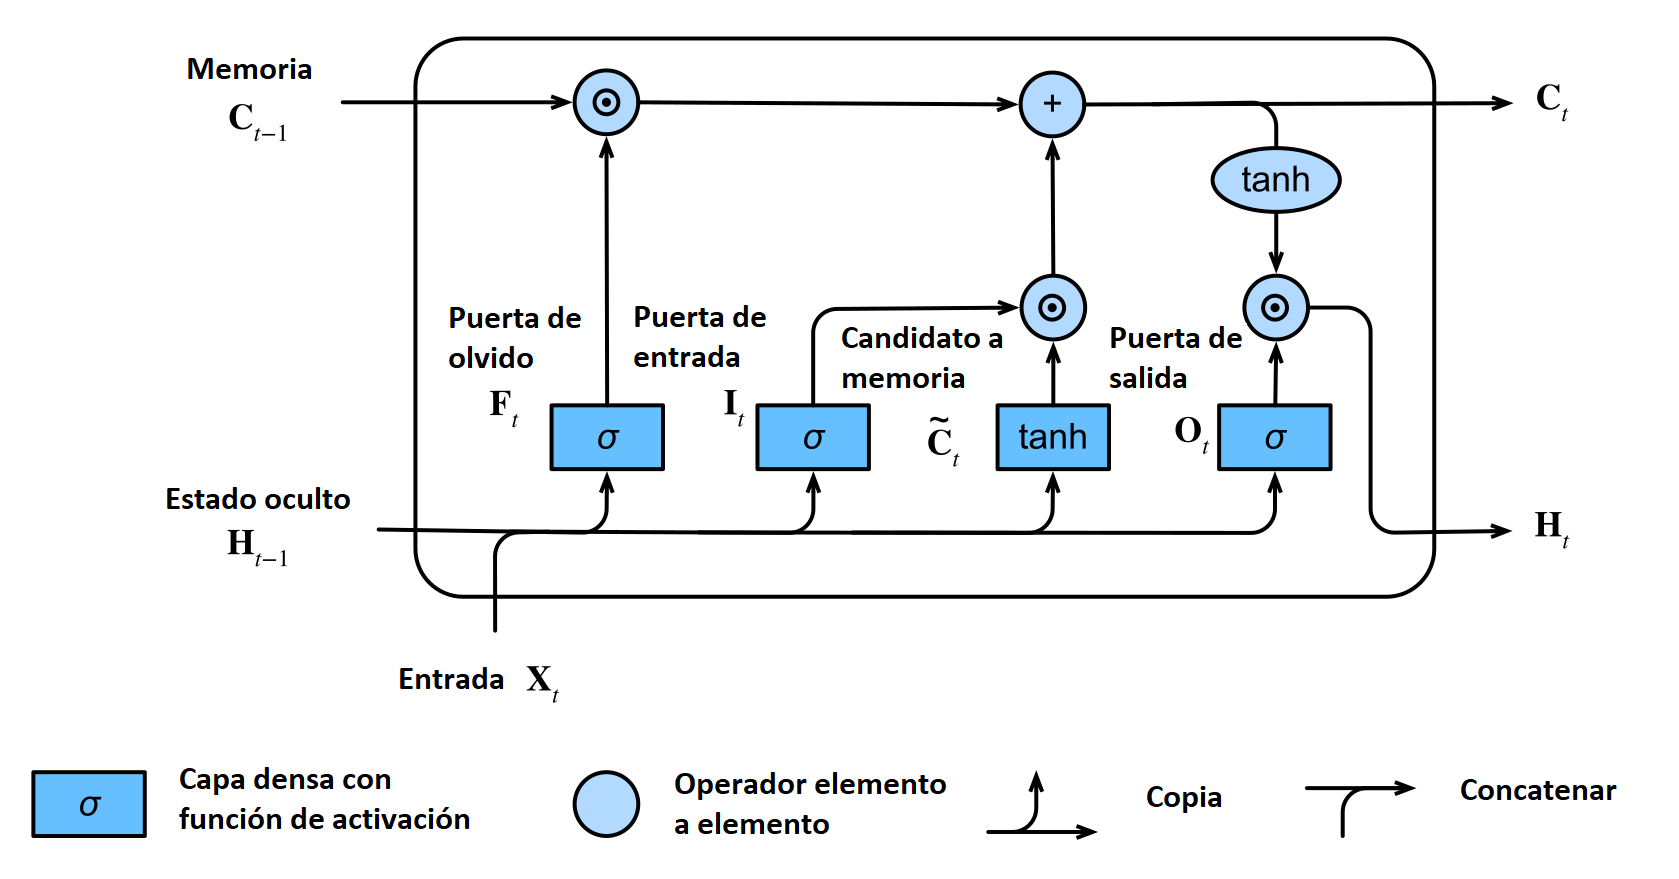
\includegraphics[scale=.4]{Graphics/rnn_lstm.png}
        \end{center}
		% TODO Cite problem, citar como texto
		% [\autocite{d2l}] 
		% [\parencite{d2l}] 
		% [\citet{d2l}] 
		% [\citep{d2l}] 
	    \caption{LSTM (Tomado de \textcite{d2l} pág. 357).}\label{fig:rnn_lstm}
	\end{center}
\end{figure}

El método de aprendizaje de las RNN solamente observa los elementos anteriores de la secuencia, aunque existen
tareas en las que, observando los elementos posteriores, se brinda más contexto e información a la tarea, sin que interfiera
en el proceso de inferencia. El modelo bidireccional presenta una alternativa para tratar con este tipo de problemas, 
este modelo consiste en, además de hacer el recorrido de inicio a final de la secuencia, realizar otro recorrido en orden 
inverso (Figura \ref{fig:rnn_bidirectional}), estos recorridos van generando dos estados ocultos $\overrightarrow{H}_{i}$ y $\overleftarrow{H}_{i}$
que luego son mezclados para obtener el contexto final $H_i$, los tipos de mezclas comunes son la concatenación de los 
estados o la multiplicación elemento a elemento de estos.

\begin{figure}[h!]
	\begin{center}
		\begin{center}
			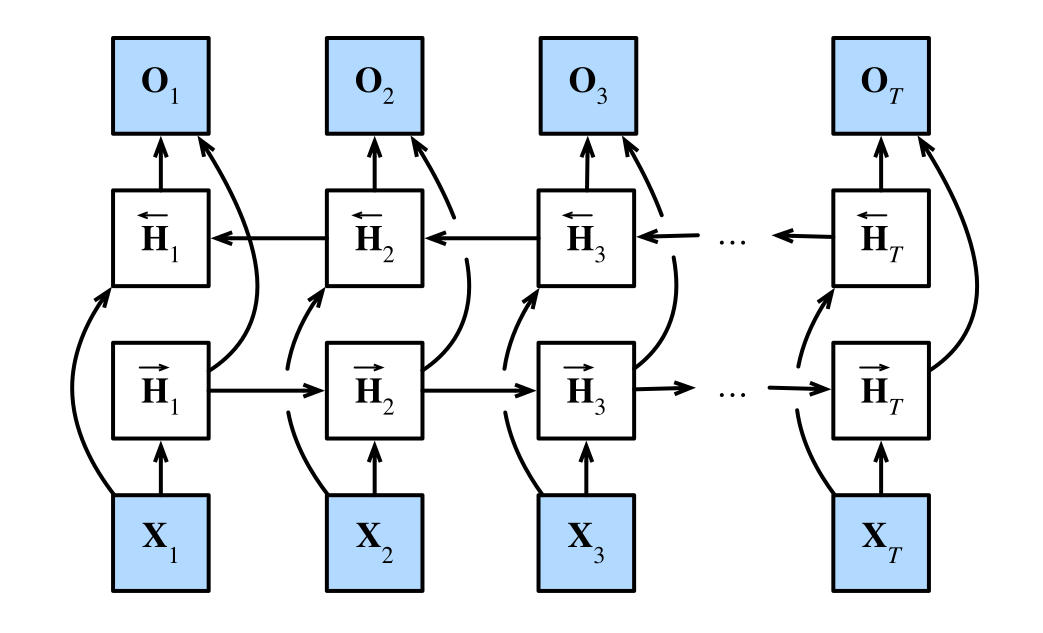
\includegraphics[scale=.3]{Graphics/rnn_bidirectional.png}
        \end{center}
		% TODO Cite problem, citar como texto
		% [\autocite{d2l}] 
		% [\parencite{d2l}] 
		% [\citet{d2l}] 
		% [\citep{d2l}] 
	    \caption{Red neuronal bidireccional (Tomado de \textcite{d2l} pág. 367).}\label{fig:rnn_bidirectional}
	\end{center}
\end{figure}


\subsubsection{Atención}

% Definicion, qué hace, uso en secuencias
La atención es una técnica en la cual se hace una selección ponderada de atributos en un contexto específico. 
Este mecanismo presenta dos partes, una consulta $q$ y una colección de pares llave-valor, $(k_i, v_i)$. La 
consulta representa el contexto en donde se quiere aplicar la atención y las llaves $k_i$ son elementos que 
relacionan la consulta a los valores $v_i$. El proceso de calcular el resultado consiste en, primero, calcular 
el vector compatibilidad $e$ entre las llaves y la consulta mediante la función $f$, este vector es luego 
modificado por una función $g$ que distribuye los valores obteniendo el vector atención $a$. Finalmente 
este vector es utilizado para calcular el resultado final al aplicarle la función $o = z(a, V)$:

\begin{equation}
	e = f(q, K),
\end{equation}
\begin{equation}
	a = g(e),
\end{equation}
\begin{equation}
	o = z(a, V).
\end{equation}

En dependencia de cómo se seleccionen las funciones $f$, $g$ y $z$ se pueden obtener distintos tipos de atención.
Una configuración simple consiste en definir $f$ como el producto punto de la consulta con la llave,
$g$ como \emph{softmax} y $z$ la suma ponderada de $v_i$ con los valores de atención.

\subsubsection{Campo Aleatorio Condicional}

% Definicion de CRF, qué modela, Ventajas de CRF en secuencias, mirar relacion con Hidden Markov Models

El campo aleatorio condicional (CRF, en inglés) es un 
tipo de modelo gráfico probabilístico que trabaja eficientemente con secuencias,
% TODO PREGUNTAR {modelando} se cambia para s y luego de {conjuntamente} se se pone con? 
modelando conjuntamente la probabilidad de las etiquetas de sus elementos dadas sus observaciones [\cite{lafferty2001conditional}].
En trabajos de secuencias, la forma más simple que toma el grafo consiste en una cadena de las variables representando
las etiquetas de las secuencias $Y$, conectadas de la forma $(Y_i, Y_{i+1})$ y las variables observadas $X$, conectadas
a las variables $Y$ [\cite{wallach2004conditional}].

El objetivo de CRF es calcular la secuencia $Y^*$ tal que:

\begin{equation}
	Y^* = \arg \max_Y P(Y | X).
\end{equation}\label{eq:crf}

En esta expresión se observa que devuelve la secuencia más probable, dadas las variables observadas o atributos $X$,
por lo que esta capa es usada al final del proceso para problemas de clasificación de secuencias.

\subsection{Evaluación del modelo y métricas}

Los modelos de AA necesitan maneras de expresar qué tan buenos son 
en las tareas encomendadas. Para esto se crean funciones que evalúan los resultados obtenidos
por dichos modelos, estas funciones se les da el nombre de métricas. Existen diferentes tipos de
métricas para tratar con diferentes tipos de problemas. En aprendizaje supervisado una métrica se
define como una función $m_s(Y, \hat{Y})$, donde $Y$ son las predicciones verdaderas y $\hat{Y}$ son las predicciones
hechas por el modelo. En algoritmos de aprendizaje no supervisado como K-Means y K-NN son usadas funciones $m_{ns}(\hat{Y})$
donde $\hat{Y}$ son las predicciones finales. En comparación con su versión supervisada estas funciones no tiene acceso
a las predicciones verdaderas del problema.

\subsubsection{Clasificación}

En problemas de clasificación (problemas en donde las etiquetas a predecir son discretas) 
son empleadas medidas que toman en cuenta la naturaleza discreta de su conjunto imagen.
Medidas como precisión, recobrado, \emph{accuracy} y F1 son utilizadas en la 
evaluación de los resultados, mientras que como función de error se usa entropía cruzada 
(\emph{cross entropy} en inglés) [\cite{grandini2020metrics}].

La matriz de confusión es una vía de representar los resultados de dos clasificadores. Esta matriz en $M_{ij}$ 
indica la cantidad de elementos que clasificó como clase $i$ el primer clasificador y
como clase $j$ el segundo clasificador. En su uso práctico,
un clasificador son las etiquetas verdaderas mientras que el otro es el clasificador que se está evaluando. 
En problemas de la clasificación binaria, donde se busca saber si existe pertenencia o no de un elemento a una clase,
se pueden observar los siguientes casos:

\begin{itemize}
	\item Verdaderos Positivos (VP): elementos clasificados correctamente que pertenecen a la clase.
	\item Verdaderos Negativos (VN): elementos clasificados correctamente que no pertenecen a la clase.
	\item Falsos Positivos (FP): elementos que no pertenecen a la clase clasificados incorrectamente en que pertenecen.
	\item Falsos Negativos (FN): elementos que pertenecen a la clase clasificados incorrectamente en que no pertenecen.
\end{itemize}

\begin{table}[h!]
	\begin{center}
		\begin{tabular}{|c|c|c|} \hline
		Clases		& Positivo	& Negativo  \\ \hline
		Positivo	& VP  		& FN		\\ \hline
		Negativo	& FP		& VN		\\ \hline
		\end{tabular}
	\caption{Matriz de confusión binaria.}\label{fig:confusion_matrix}
	\end{center}
\end{table}

La precisión es la medida que indica la probabilidad de que la clasificación de una clase sea correcta. Esto 
se puede observar como la proporción de los elementos correctamente clasificados sobre el total de 
elementos clasificados:

\begin{equation}
	prec_i = \frac{VP}{VP + FP}.
\end{equation}

En problemas de clasificación múltiple surge la versión macro de esta medida calculada como la media de todas
las precisiones de las clases existentes:

\begin{equation}
	prec_{macro} = \sum^K_{i=1} \frac{prec_i}{K}.
\end{equation}

El recobrado es la medida que indica la probabilidad de que se clasifique correctamente un elemento de la clase
del total existente. Esto se puede observar como la proporción de los elementos correctamente clasificados sobre el 
total de elementos que pertenecen a la clase:

\begin{equation}
	rec_i = \frac{VP}{VP + FN}.
\end{equation}

En problemas de clasificación múltiple surge la versión macro de esta medida calculada como la media de todos
los recobrados de las clases existentes:

\begin{equation}
	rec_{macro} = \sum^K_{i=1} \frac{rec_i}{K}.
\end{equation}

La medida F1 es la media armónica de la precisión y el recobrado. En esta la contribución de la precisión y el
recobrado al resultado final es el mismo, aunque es posible buscar variaciones de acuerdo a al problema a tratar:

\begin{equation}
	F1_i = 2 \frac{prec_i \cdot rec_i}{prec_i + rec_i}.
\end{equation}

En problemas de clasificación múltiple surge la versión macro de esta medida calculada la propia medida F1, pero
utilizando la precisión y recobrado macro del problema:

\begin{equation}
	F1_{macro} = 2 \frac{prec_{macro} \cdot rec_{macro}}{prec_{macro} + rec_{macro}}.
\end{equation}

La métrica $\alpha$\%F1 [\cite{persing2016end}] es una métrica basada en la idea de F1 orientada para el 
trabajo con secuencias donde $\alpha$ denota el porcentaje de secuencia inferida que debe coincidir con 
la secuencia anotada para ser considerado una coincidencia. Esta versión permite
establecer el rango de flexibilidad si $\alpha=100$ (100\%F1), significa que deben coincidir completamente, 
mientras si $\alpha = 50$ (50\%F1) significa que, si coinciden en una proporción mayor o igual a la mitad, 
se considera como un verdadero positivo. La definición de los valores de verdaderos positivos, negativos 
y falsos negativos es:

\begin{equation}
	VP = |\{ j | \exists i | gl(j) = pl(i) \land i = j \}|,
\end{equation}
\begin{equation}
	FP = |\{ i | pl(i) \neq n \land \not\exists j | gl(j) = pl(i) \land i = j \}|,
\end{equation}
\begin{equation}
	FN = |\{ j | \not\exists i | gl(j) = pl(i) \land i = j \}|,
\end{equation}

donde $i$ y $j$ son las UDAs extraídas, $gl(j)$ es la etiqueta correcta para $j$, $pl(i)$ es 
la etiqueta inferida para $i$, $n$ es la clase no argumentativa, $i = j$ significa que $i$ es 
una coincidencia para $j$.

Las métricas anteriores están acotadas por los valores 0 y 1, donde 1 representa la mejor evaluación y 0 la 
peor.

La entropía cruzada se encarga de evaluar qué tan diferentes son dos funciones de distribución $p$ y $q$, su 
resultado es un número no negativo que, a medida que sean más pequeños los valores, indican mayor similitud. 
En su versión discreta se formula así:

\begin{equation}
	H(p, q) = - \sum_{x \in D} p(x) \log q(x).
\end{equation}

\subsubsection{Cadenas}

Para textos o cadenas existen diferentes métricas que constituyen formas de saber la similitud 
entre dos elementos. Una de esas métricas es la similitud de Jaccard, esa se puede ver como 
la proporción de elementos comunes que presentan dos conjuntos, los elementos sería palabras:

\begin{equation}
	jac(X, Y) = \frac{|X \cap Y|}{|X \cup Y|}.
\end{equation}
Otra medida de similitud es la distancia de Levenshtein, la cual se define como la mínima cantidad 
de cambios de eliminar, cambiar y agregar que se tienen que hacer a dos secuencias para que sean 
iguales. Esta medida se puede usar tanto en palabras, en donde se mediría la cantidad de cambios 
a los caracteres, como en listas de palabras, donde se mediría la cantidad de palabras que 
se tienen que cambiar. 

\subsubsection{Curvas de aprendizaje}

Es necesario además de evaluar el resultado final del modelo, evaluar el proceso de entrenamiento. En esta etapa 
se pueden diagnosticar varias deficiencias en este proceso. Para un correcto entrenamiento se divide el conjunto de 
datos en tres partes:

\begin{itemize}
	\item \textbf{entrenamiento}: utilizada para el entrenamiento del modelo.
	\item \textbf{validación}: utilizada para evaluar el desempeño del modelo durante el entrenamiento.
	\item \textbf{prueba}: utilizada para evaluar el resultado final.
\end{itemize}

Las curvas de aprendizaje constituyen la principal herramienta para evaluar el proceso de aprendizaje.
Estas están formadas por las mediciones de métricas a lo largo del entrenamiento calculadas a partir de 
los conjuntos de validación y entrenamiento. En estas, el eje horizontal representa el número de época del entrenamiento,
iteración sobre el conjunto de entrenamiento, y el eje vertical representa el valor de la métrica a analizar. 
La línea correspondiente al conjunto de entrenamiento cuantifica 
el aprendizaje del modelo o también el error de entrenamiento, y la correspondiente a la de validación cuantifica 
la generalización o el error de generalización. Existen tres comportamientos esenciales a analizar:

\begin{itemize}
	\item Bajo ajuste (\emph{underfitting}).
	\item Sobreajuste (\emph{overfitting}).
	\item Buen ajuste.
\end{itemize}

El bajo ajuste ocurre cuando el modelo no es capaz de aprender del conjunto de datos o cuando este aún puede aprender 
más. Las curvas de aprendizaje en estos casos se caracterizan por ser una línea plana o valores ruidosos con alta pérdida
(Figura \ref{fig:underfit}).

\begin{figure}[h!]
	\begin{center}
		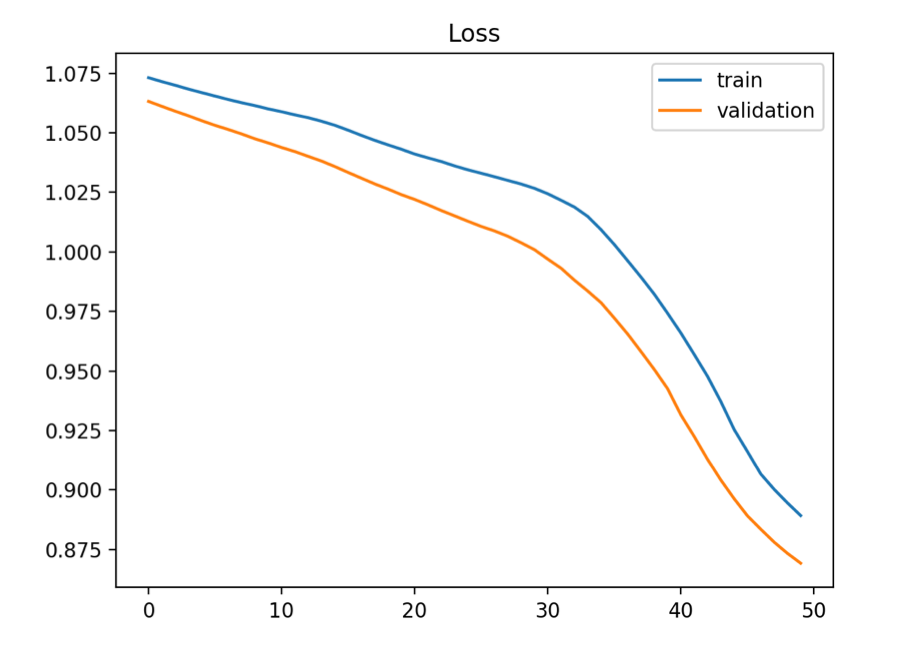
\includegraphics[scale=.2]{Graphics/underfit_missing_training.png}
		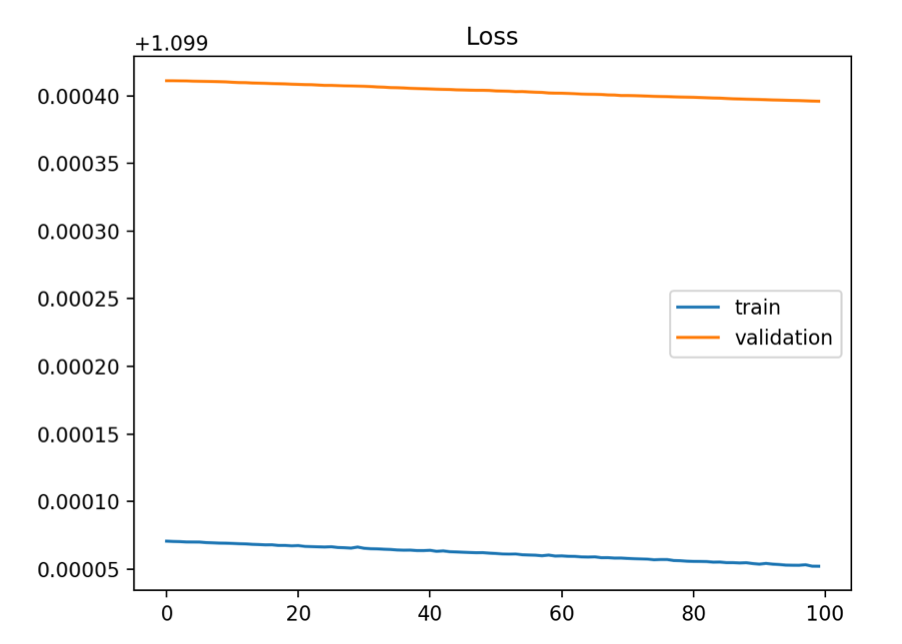
\includegraphics[scale=.2]{Graphics/underfit_not_learning.png}
		% TODO Cite problem, citar como texto
		% TODO PREGUNTAR, la página es en romano, luego de esas vienen páginas en números normales,
		% poner el número normal traería confusión
		% [\autocite{brownlee2018better}] 
		% [\parencite{brownlee2018better}] 
		% [\citet{brownlee2018better}] 
		% [\citep{brownlee2018better}] 
		\caption{Curvas de entrenamiento con bajo ajuste por falta de entrenamiento (izquierda) 
		y por modelo que no aprende de los datos (derecha) (Tomado de \textcite{brownlee2018better} pág. XXVII).}\label{fig:underfit}
	\end{center}
\end{figure}

Entre las formas más sencillas de combatir el bajo ajuste de los modelos consiste en complejizarlo, al añadir
capas o aumentar las dimensiones de este aumenta su expresividad y, por lo tanto, su ajuste. Si este método 
no funciona es posible considerar un cambio de arquitectura hacia una que pueda extraer más información de la 
estructura de los datos. 

El sobreajuste es el fenómeno en el que el modelo aprende los datos de entrenamiento extremadamente bien, incluso
el ruido en estos, esto trae consigo que falla en generalizar el problema para nuevas entradas. Las curvas 
características de este fenómeno presentan una divergencia en los errores de entrenamiento y validación a medida
que se entrena el modelo, mientras que la de entrenamiento mejora la de validación tiende a empeorar (Figura \ref{fig:overfit}). 

\begin{figure}[h!]
	\begin{center}
		\begin{center}
			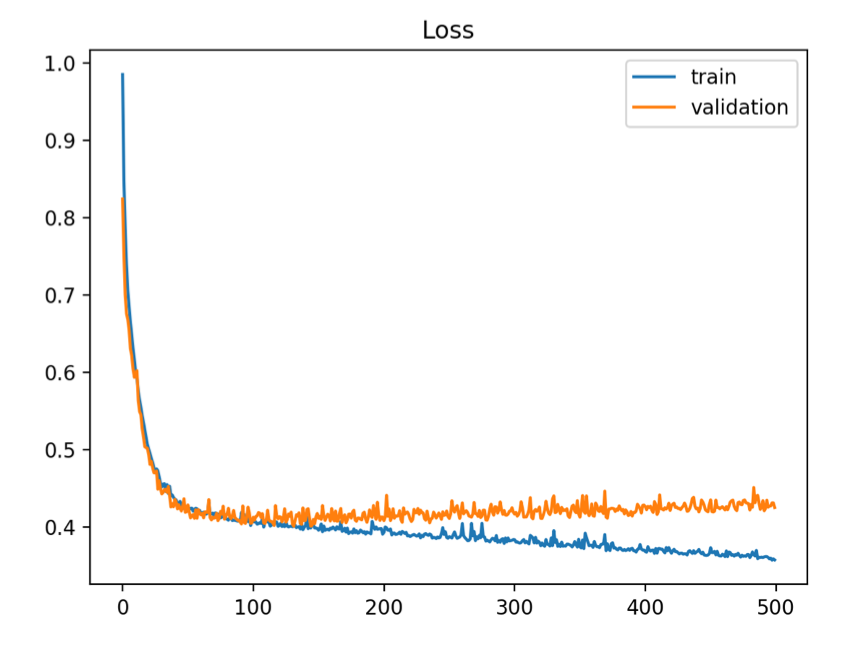
\includegraphics[scale=.3]{Graphics/overfit_raising_val_error.png}
        \end{center}
		% TODO Cite problem, citar como texto
		% TODO PREGUNTAR, la página es en romano, luego de esas vienen páginas en números normales,
		% poner el número normal traería confusión
		% [\autocite{brownlee2018better}] 
		% [\parencite{brownlee2018better}] 
		% [\citet{brownlee2018better}] 
		% [\citep{brownlee2018better}] 
	    \caption{Curvas de entrenamiento con sobreajuste (Tomado de \textcite{brownlee2018better} pág. XXIX).}\label{fig:overfit}
	\end{center}
\end{figure}

Existen varios métodos para combatir el sobreajuste, uno sencillo es simplificar el modelo quitándole capas 
o disminuyendo sus dimensiones. Además de esto, existen regularizaciones que se pueden aplicar para evitar que 
las capas dependan exclusivamente de pocos atributos, entre esta familia los más usados son la regularización
L1 y L2 las cuales se definen como la suma del valor absoluto de los atributos y la suma del cuadrado de sus 
atributos respectivamente. Otra medida para prevenir el sobreajuste es el agrego de capas de abandono 
(\emph{dropout}). Estas capas desactivan neuronas de la arquitectura, obligando a 
estas a ser robustas y depender del comportamiento de la población, en lugar de la actividad de otras unidades 
específicas [\cite{baldi2013dropout}]. La terminación temprana (\emph{early stopping}) del entrenamiento
se utiliza para parar este en el momento en que el error de generalización comienza a subir, impidiendo así que 
se sobreentrene el modelo.

Finalmente, un buen ajuste es el resultado que se alcanza cuando tanto la curva de validación como de entrenamiento
presentan valores pequeños y similares, consecuentes con una correcto aprendizaje y generalización (Figura \ref{fig:good_fit}).

\begin{figure}[h!]
	\begin{center}
		\begin{center}
			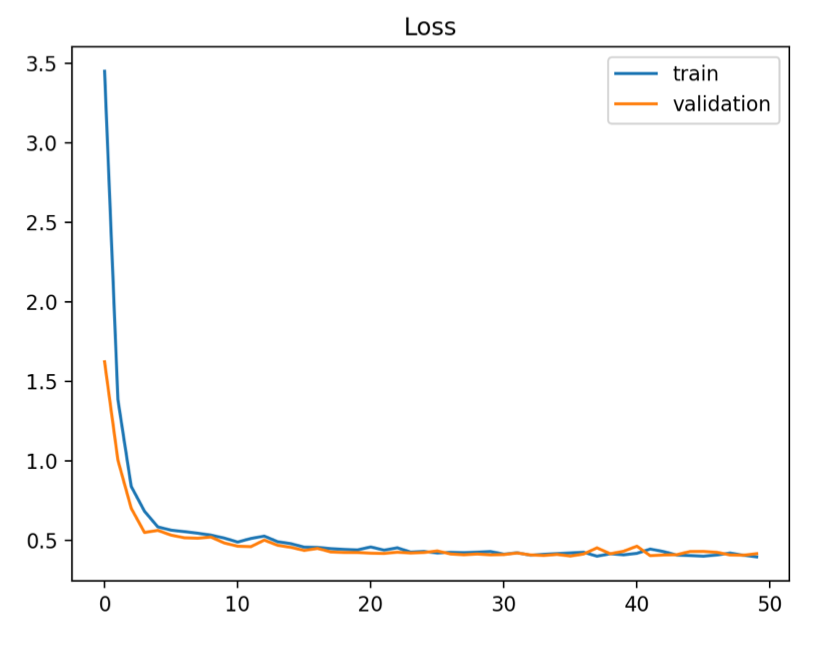
\includegraphics[scale=.3]{Graphics/good_fit.png}
        \end{center}
		% TODO Cite problem, citar como texto
		% TODO PREGUNTAR, la página es en romano, luego de esas vienen páginas en números normales,
		% poner el número normal traería confusión
		% [\autocite{brownlee2018better}] 
		% [\parencite{brownlee2018better}] 
		% [\citet{brownlee2018better}] 
		% [\citep{brownlee2018better}] 
	    \caption{Curvas de entrenamiento con buen ajuste (Tomado de \textcite{brownlee2018better} pág. XXX).}\label{fig:good_fit}
	\end{center}
\end{figure}

Otro problema observable a partir del análisis de las curvas de aprendizaje constituye la detección de conjuntos
de datos no representativos. Un conjunto de datos no representativo es uno que puede no 
capturar las características estadísticas relativas a otro conjunto de datos extraído del mismo dominio.
Esto puede pasar que los conjuntos de entrenamiento o de validación. En caso del conjunto de entrenamiento
se puede identificar si la pérdida en el conjunto de entrenamiento conlleva a una ganancia en el conjunto de 
validación y viceversa quedando al final con una separación entre ambos valores. En el caso del conjunto de 
validación se presenta como una curva ruidosa, también se puede dar el caso de que el conjunto  de validación
sea más fácil de predecir que el de entrenamiento, en este caso se observa como la curva de validación permanece
siempre por debajo de la de entrenamiento (Figura \ref{fig:unrepresentative_data}).

\begin{figure}[h!]
	\begin{center}
		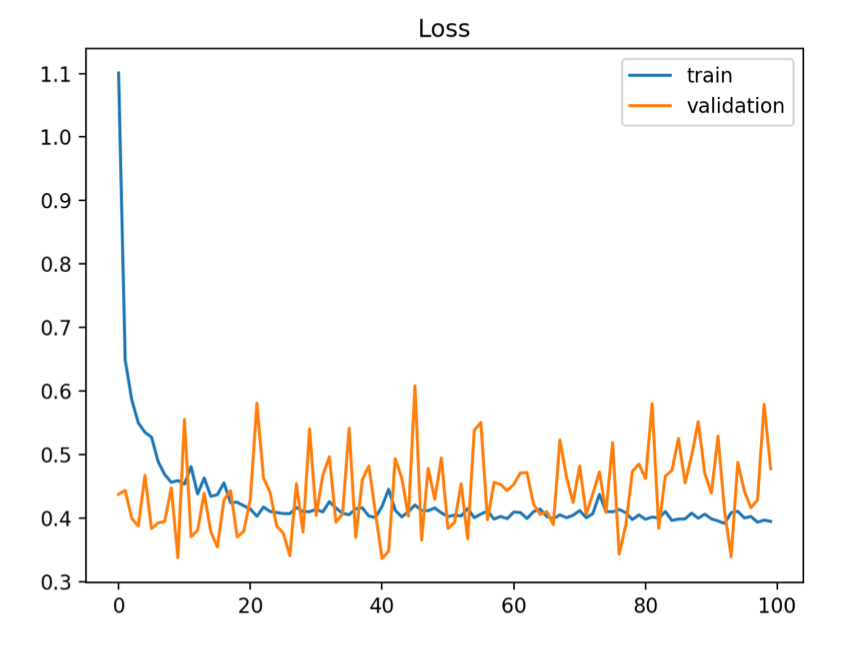
\includegraphics[scale=.2]{Graphics/unrepresentative_dev_set.png}
		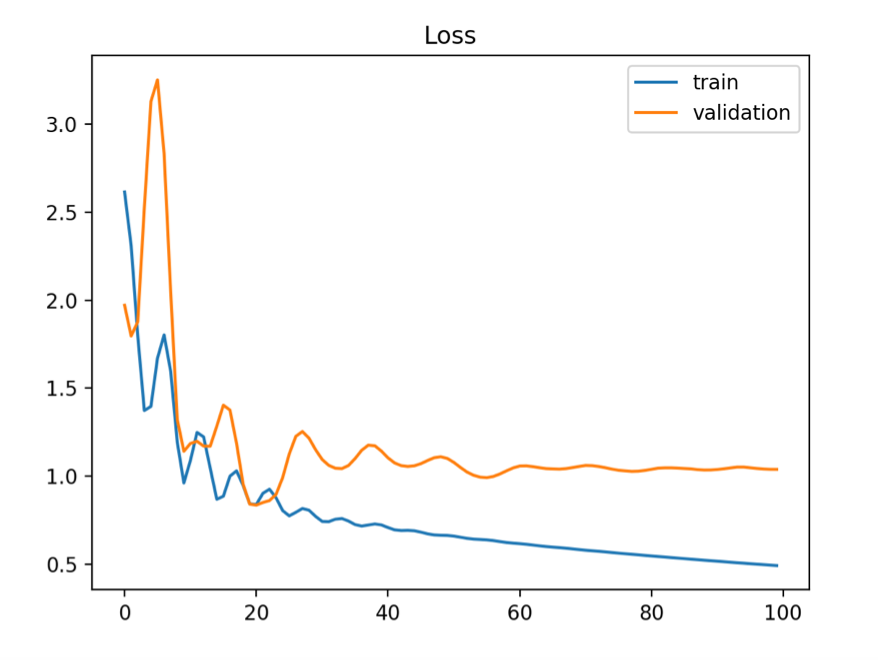
\includegraphics[scale=.2]{Graphics/unrepresentative_train_set.png}
		% TODO Cite problem, citar como texto
		% TODO PREGUNTAR, la página es en romano, luego de esas vienen páginas en números normales,
		% poner el número normal traería confusión
		% [\autocite{brownlee2018better}] 
		% [\parencite{brownlee2018better}] 
		% [\citet{brownlee2018better}] 
		% [\citep{brownlee2018better}] 
		\caption{Curvas de entrenamiento con datos poco representativos en el conjunto de validación (izquierda) 
		y en el conjunto de entrenamiento (derecha) (Tomado de \textcite{brownlee2018better} pág. XXXII).}\label{fig:unrepresentative_data}
	\end{center}
\end{figure}

Para combatir estos problemas se puede aumentar la cantidad de elementos en los conjuntos de entrenamiento o 
validación en dependencia de donde ocurra.

\subsection{Aumento de datos}

El aumento de datos consiste en acciones para aumentar la diversidad de un conjunto de datos sin recolectar
nuevos datos explícitamente [\cite{feng2021data}]. En datos continuos, como imágenes o valores numéricos el 
aumento de datos puede ser realizado al añadirle perturbaciones a entradas existentes, en caso de las imágenes 
técnicas como el volteado (\emph{flipping}) o recortado (\emph{cropping}) son usadas. Los textos son un tipo 
de datos discreto y, por lo tanto, las técnicas anteriores no pueden ser aplicadas directamente. Para el PLN
se han estudiado diversas técnicas de aumento de datos, una de estas consiste en el cambio del árbol de 
dependencia de la oración mediante operaciones de intercambio y borrado de nodos [\cite{csahin2019data}], también se han utilizado 
el intercambio de palabras por sinónimos [\cite{dai2020analysis}] y la traducción de textos hacia un lenguaje y luego 
de vuelta al lenguaje origen (\emph{backtranslation}) [\cite{sennrich2015improving}]. 

\subsection{Aprendizaje Conjunto}

El aprendizaje conjunto (\emph{ensemble learning}) son técnicas encaminadas al aprovechamiento
de soluciones encontradas por diferentes modelos, combinándolas y mejorándolas para encontrar una mejor solución 
al problema. Estos métodos son efectivos en la reducción de la varianza y el sesgo de los modelos, obteniendo así
mejores resultados [\cite{dietterich2002ensemble}]. Una forma de este tipo de aprendizaje en problemas de 
clasificación constituye el voto conjunto, en donde los diferentes clasificadores votan sobre la clase a la que 
pertenece el elemento y, al final, se asigna la etiqueta que más votos obtuvo.

\subsection{Métodos de optimización}

El objetivo del AA es encontrar los extremos de una función de costo, este proceso es una tarea 
desafiante ya que la gran mayoría de estas funciones no son convexas y, por lo tanto, no existe un algoritmo
que asegure la convergencia hacia un extremo global. Para resolver este problema existen múltiples heurísticas,
la más usada es el descenso por gradiente. La idea básica consiste 
en el cálculo del vector gradiente de la función de error $f$ con respecto a los parámetros del modelo $x$ y, una vez se 
tiene dicho vector, se evalúa en la asignación actual de los parámetros $x_i$ y se realiza un corrimiento de este punto 
% TODO PREGUNTAR dice sustituir por {dirección} contra. No debe ser así no? 
en contra del gradiente para disminuir el error (Eq. \ref{eq:gradien_descent}).

\begin{equation}
	x_{i+1} = x_i - \alpha \nabla f(x_i)\label{eq:gradien_descent}
\end{equation}

En la ecuación \ref{eq:gradien_descent} anterior, $\alpha$ es la tasa de aprendizaje (\emph{learning rate}),
que cuantifica cuánto se toma del vector de gradiente para actualizar los parámetros, esto 
se puede ver como el aprendizaje del modelo.

Variantes eficientes de este algoritmo para el entrenamiento de modelos de AA han sido 
creadas, las variaciones se encuentran principalmente en la selección de $\alpha$ en cada paso y la 
selección de los conjuntos de datos con que se estimará el gradiente. Entre las técnicas utilizadas se 
encuentran Descenso por Gradiente Estocástico, variaciones de tasa de aprendizaje dinámica con 
sus diferentes variantes (exponencial, polinómica), RMSProp [\cite{tieleman2012rmsp}] 
y Adam [\cite{kingma2014adam}].

\section{Preliminares de Extracción de Argumentos}

Varias investigaciones han dado respuesta a los problemas asociados a EA, mostrando
una variedad en enfoques y métodos.

% TODO Cite problem, citar como texto
% [\autocite{palau2009argumentation}] 
% [\parencite{palau2009argumentation}] 
% [\citet{palau2009argumentation}] 
% [\citep{palau2009argumentation}] 
En \textcite{palau2009argumentation} se propone
el uso de modelos estadísticos como \emph{Naive Bayes} (NB) y \emph{Support Vector Machine} (SVM) 
para la clasificación de 
oraciones en argumentativas o no y en su rol argumentativo en caso de que sea argumentativa. En este
se asume que las componentes argumentativas son oraciones completas. Para la predicción de relaciones
se usa un enfoque basado en reglas con la creación de una Gramática Libre de Contexto. Las representaciones
de las oraciones consisten en atributos creados a mano, dado el conocimiento experto sobre la argumentación
en el tema tratado, elementos como adverbios, verbos, signos de puntuación, palabras clave, estadísticas del texto
(tamaño de oración, distancia media de palabras) son usados para la extracción y clasificación de las UDAs, además,
se usan también como base en la creación de las reglas de la gramática para la extracción de relaciones.

% TODO Cite problem, citar como texto
% [\autocite{goudas2015argument}] 
% [\parencite{goudas2015argument}] 
% [\citet{goudas2015argument}] 
% [\citep{goudas2015argument}] 
\textcite{goudas2015argument} al igual que \textcite{palau2009argumentation} clasifica a las oraciones como
argumentativas o no, mediante diferentes clasificadores como NB, \emph{Random Forest}, Regresión
Logística y SVM. Sin embargo, \textcite{goudas2015argument} aumenta la grandularidad de la segmentación al permitir
la extracción de los segmentos que contienen la carga argumentativa de dentro de las oraciones previamente clasificadas
como tal, esto se realiza mediante la extracción de etiquetas BIO de las oraciones con el uso de un 
CRF. La predicción de las relaciones es modelado como un problema de clasificación
% TODO PREGUNTAR dice eliminar {en}, pero no le veo el sentido a eso.
usando SVM para clasificar pares de UDAs en relacionados o no. Atributos creados a mano 
son usados en la extracción de UDAs; entre estos están posición de la oración en el texto, cantidad de verbos, comas, adverbios,
palabras, entidades en la oración, también se emplean listas que guardan entidades relacionadas con el dominio 
específico y palabras clave indicadoras de frases argumentativas. 

% TODO Cite problem, citar como texto
% [\autocite{stab2017parsing}] 
% [\parencite{stab2017parsing}] 
% [\citet{stab2017parsing}] 
% [\citep{stab2017parsing}] 
\textcite{stab2017parsing} proponen un mecanismo de segmentación basado en CRF. La clasificación
y predicción de relaciones se modela conjuntamente con dos clasificadores SVM y un problema
de Optimización Lineal Entero que encuentra la mejor estructura y asegura una disposición arbórea. En la segmentación
de las UDAs, se extraen por cada token su posición en el texto, si precede o sucede a un signo de puntuación, su parte de
la oración, la probabilidad de que sea el comienzo de una UDA dado sus tokens anteriores, entre otros. Para la extracción
y clasificación de relaciones se proponen otros conjuntos de atributos como la cantidad de sustantivos comunes entre
las componentes fuente y el objetivo, la presencia de indicadores argumentativos, representaciones vectoriales de tokens,
entre otros.

% TODO Cite problem, citar como texto
% [\autocite{eger2017neural}] 
% [\parencite{eger2017neural}] 
% [\citet{eger2017neural}] 
% [\citep{eger2017neural}] 
En \textcite{eger2017neural} trabajan el problema de EA como uno \emph{end-to-end}. 
Para esto presentaron varias propuestas, entre ellas se encontraba
modelar el problema como uno de secuencia a secuencia, usando RNN como 
LSTM en versiones bidireccionales capturando información desde ambos lados de la secuencia.
Para la representación de las palabras se extrajo información morfológica de las palabras mediante 
la aplicación de una CNN a los caracteres de estas,
al final, realizan la clasificación de la secuencia con un CRF. 
Realizaron experimentos al modelar el problema como uno de \emph{Dependency Parsing} [\cite{kiperwasser2016simple}]. Este problema
consiste en construir un árbol de dependencia que codifique las estructuras argumentativas. En este 
se tiene que decidir entre varias opciones (\emph{shift}, \emph{reduce}) en dependencia del contenido de la pila y del \emph{buffer}
para la confección del árbol.
El problema fue modelado también como un problema de reconocimiento de entidades nombradas, en donde las entidades son las UDAs.

% TODO Cite problem, citar como texto
% [\autocite{dykes2020reconstructing}] 
% [\parencite{dykes2020reconstructing}] 
% [\citet{dykes2020reconstructing}] 
% [\citep{dykes2020reconstructing}]
En \textcite{dykes2020reconstructing} se proponen métodos basados en reglas para la extracción de argumentos sobre
textos en Twitter. Estos métodos se centran en la confección de reglas basadas en anotaciones lingüísticas como
partes de la oración y lemas de palabras. La recuperación está basada en los esquemas argumentativos comunes presentes
en los textos. Dada las reglas creadas y el tipo
de datos con que se trabaja, o sea, cadenas de texto pequeñas; estos algoritmos tienden a tener una alta precisión aunque 
bajo recobrado, esto no es un gran problema en conjuntos de datos grandes, pero en conjuntos de menor tamaño o estructura 
más compleja pierden efectividad.

% TODO Cite problem, citar como texto
% [\autocite{galassi2021deep}] 
% [\parencite{galassi2021deep}] 
% [\citet{galassi2021deep}] 
% [\citep{galassi2021deep}]
\textcite{galassi2021deep} propone el uso de redes residuales y mecanismos de atención
para la creación de un modelo que, conjuntamente, clasifica el tipo de UDA y la relación existente entre estas.
Este trabajo define el concepto de distancia argumentativa, añadiéndolo como característica y asume que las UDAs ya fueron 
extraídas. En este caso, además de la distancia argumentativa, las secuencias son representadas 
vectorialmente con GloVe.

En resumen, se contemplan disímiles enfoques al problema de EA desde una perspectiva enmarcada en modelos 
simbólicos, estadísticos y neuronales en versiones tanto secuenciales como \emph{end-to-end}. 
Cada uno de estos modelos presentan sus ventajas y desventajas a la hora de construirlos, 
extenderlos y comprender su funcionamiento. En modelos simbólicos se presenta una alta
precisión en dominios específicos debido a que se construyen teniendo en cuenta reglas específicas a un
contexto dado. Estos modelos son poco escalables y difíciles de mantener ya que sus reglas son construídas
a mano y dicho proceso requiere de conocimiento experto y tiempo. Los modelos estadísticos 
se caracterizan por usar conjuntos de atributos creados a mano, dichos atributos son difíciles
de encontrar, calcular y pueden no poseer relevancia en otros contextos diferentes a los que fueron creados,
además, la necesidad de conocimiento experto es necesaria para su confección. Los modelos neuronales poseen
una mayor adaptabilidad, en estos la entrada puede ser codificada en una representación que es aprendida por
el mismo algoritmo, permitiendo su uso en esquemas argumentativos con características diferentes. Los modelos simbólicos y 
estadísticos poseen la ventaja de poder explicar el porqué de los resultados devueltos cosa que se vuelve casi
imposible en modelos neuronales.

Dado que la EA es un proceso en el cual se necesita pasar por varias tareas, estas deben de ser completadas
de alguna forma. Una manera de completarlas es hacerla una a la vez, independiente una de otra y pasándole
la salida de etapas anteriores a las etapas siguientes. Esta manera secuencial de realizar las 
tareas es bastante simple y ayuda a la creación de modelos simples y con tareas bien definidas, aunque trae consigo 
la propagación de los errores a través del proceso y el no aprovechamiento de las interrelaciones entre variables 
computadas de procesos anteriores. También requiere de la construcción, entrenamiento y evaluación de varios modelos.
En cambio un enfoque \emph{end-to-end} poseen la habilidad de modelar el problema 
desde su inicio hasta su final de manera conjunta, mediante \emph{Multi-Task Learning} (MTL) se modelan
las tareas de manera conjunta creando un solo modelo complejo con una propagación de error menor.

\section{Proyección de corpus}

La EA no presenta una gran cantidad de datos anotados con los cuales se pueda realizar 
un entrenamiento, además de esto la gran mayoría de corpus existentes se encuentran en lenguajes como inglés o alemán,
haciendo difícil el desarrollo de esta rama en otros lenguajes.
La escasez de estos datos es, en gran parte, debida al elevado costo monetario, de tiempo y de recursos humanos que se utiliza
en su creación. En orden de poder desarrollar la EA en otros lenguajes, como el español, se han investigado diferentes vertientes
para la construcción de conjuntos de datos en estos lenguajes de pocos recursos, a partir de los conjuntos de datos ya 
existentes.

La proyección de etiquetas consiste en un algoritmo en donde se 
transfieren las etiquetas de un corpus anotado a nivel de tokens en un lenguaje origen hacia su traducción en un
% TODO Cite problem, citar como texto
% [\autocite{eger2018cross}] 
% [\parencite{eger2018cross}] 
% [\citet{eger2018cross}] 
% [\citep{eger2018cross}] 
lenguaje objetivo. En \textcite{eger2018cross} se propone un algoritmo de proyección dadas las alineaciones de 
palabras. El proceso se divide en varias partes:

\begin{enumerate}
	\item Traducción de oraciones.
	\item Alineación de palabras.
	\item Proyección de etiquetas.
\end{enumerate}

\subsection{Traducción de oraciones}

La Traducción Automática consiste en el proceso de usar inteligencia artificial para
traducir texto de un lenguaje fuente a un lenguaje objetivo sin la intervención humana.
En la actualidad, este campo ha dado un gran paso pasando de modelos estadísticos a modelos
neuronales obteniendo traducciones de una alta calidad sin variar significativamente de la humana, 
condición necesaria para una buena proyección [\cite{eger2018cross}].

Este primer paso de la proyección de corpus consiste en traducir todas las oraciones existentes 
en el conjunto de datos hacia el lenguaje objetivo. 
% TODO Cite problem, citar como texto
% [\autocite{stab2017parsing}] 
% [\parencite{stab2017parsing}] 
% [\citet{stab2017parsing}] 
% [\citep{stab2017parsing}] 
A continuación se muestra una oración en inglés y su traducción al español\footnote{Extraído del corpus de \textcite{stab2017parsing}.}:

\begin{adjustwidth}{25pt}{25pt}
	Firstly , people normally have lots of things to do . \\
	En primer lugar , la gente normalmente tiene muchas cosas que hacer .
\end{adjustwidth}

\subsection{Alineación de palabras}

La alineación de palabras consiste en encontrar las palabras generadas en el lenguaje objetivo por las 
palabras en el lenguaje fuente.
Algoritmos basado en modelos bayesianos, como FastAlign [\cite{dyer2013fastalign}], 
y Cadenas de Markov-Monte Carlo, como EFEMARAL [\cite{ostling2016efficient} se ubican entre
las primeras herramientas para la solución del problema. 
Modelos más recientes se han enfocado en explotar las representaciones
vectoriales de palabras y el uso de métodos de atención para la extracción de las
alineaciones [\cite{dou2021word}]. Algunas consideraciones sobre el proceso: las relaciones 
formadas entre palabras pueden ser de tipo muchos a muchos, además de no tener el mismo orden de la 
oración inicial o incluso no estar relacionadas directamente con una palabra en la oración objetivo.
Estas consideraciones dan una medida de la dificultad de la tarea en cuestión.
En el ejemplo siguiente se observa el resultado de las herramientas de alineación, en este 
las palabras en el idioma de origen (inglés) están anotadas con su posición en la oración y 
las palabras en el idioma objetivo (español) están anotadas con la posición de la palabra que 
la originó en el idioma origen:

\begin{adjustwidth}{25pt}{25pt}
	Firstly$_0$ ,$_1$ people$_2$ normally$_3$ have$_4$ lots$_5$ of$_6$ things$_7$ to$_8$ do$_9$ .$_{10}$ \\
	En primer$_0$ lugar$_0$ ,$_1$ la gente$_2$ normalmente$_3$ tiene$_4$ muchas$_5$ cosas$_7$ que$_8$ hacer$_9$ .$_{10}$
\end{adjustwidth}

\subsection{Proyección de etiquetas}

La proyección de etiquetas consiste en transportar las etiquetas de las palabras en la secuencia origen
hacia las palabras de la secuencia destino tomando como datos las alineaciones entre estas. En [\cite{yarowsky2001inducing}]
se trata el problema de proyección de frases nominales, estas frases tienen como característica que son resistentes
a ser divididas en caso de ser traducidas, y aunque evidencian 
cambios en el orden de las palabras, mantienen la misma ventana; dicha propiedad se cumple para las UDAs también.
La proyección de UDAs es más simple en dado
que solamente se tiene en cuenta la ventana y las etiquetas en estas son constantes, no pasa con la proyección en
frases nominales, las cuales pueden cambiar dentro de una ventana, por lo que algoritmos más simples existen
para esta tarea [\cite{eger2018cross}]. En el ejemplo de proyección están anotadas las etiquetas originales en formato BIO
de las palabras de la oración en el lenguaje origen (inglés) y se muestra el
resultado de proyectar estas al lenguaje objetivo utilizando los resultados de la alineación de palabras:

\begin{adjustwidth}{25pt}{25pt}
	Firstly$_O$ ,$_O$ people$_B$ normally$_I$ have$_I$ lots$_I$ of$_I$ things$_I$ to$_I$ do$_I$ .$_O$ \\
	En$_O$ primer$_O$ lugar$_O$ ,$_O$ la$_O$ gente$_B$ normalmente$_I$ tiene$_I$ muchas$_I$ cosas$_I$ que$_I$ hacer$_I$ .$_O$
\end{adjustwidth}
